\section{Fuzzy Systems}

\subsection{Introduction to fuzzy logic}

What's the \textbf{motivation} behind the use of \textbf{fuzzy logic}? Humans use imprecise linguistic terms and make complex reasoning based on that terms, classical mathematics cannot manage these terms. To use these terms with computer we have fuzzy logic.\\

\subsubsection{Imprecision and Uncertainty}

Any \textbf{notion} is said to be \textbf{imprecise} when its meaning is not fixed, something more than \textit{true} or \textit{false}, the value can be in between, there's a \textbf{gradualness}, also called \textbf{fuzziness}.\\

A \textbf{proposition} is \textbf{imprecise} if it contains \textbf{gradual predicates}, propositions true to a certain degree.\\

Sorites \textbf{paradox}: if a sand dune is small, adding one grain of sand to it leaves it small, a sand dune with a single grain is small, hence all sand dunes are small. What's the threshold for a sand dune?\\
Formulation:
\begin{itemize}
	\item Statement $A(n):$ "$n$ grains of sand are a sand dune"
	\item Let $d_n = T(A(n))$ denote the \textbf{degree of acceptance} for $A(n)$
	\item Then $0 = d_0 \leq d_1 \leq \, \dots \, \leq d_n \leq \, \dots \, \leq 1$ can be seen as \textbf{truth values of a many-valued logic} 
\end{itemize}
There's no definite threshold, there must be different degrees (e.g. the difference between "slow" and "fast" is not 1km/h).\\

Fuzzy set theory \textbf{does not assume any threshold} (no discrete thresholds at least).\\

\newpage

\paragraph{Difference between imprecision and uncertainty:} They're not the same: 
\begin{itemize}
	\item \textbf{Imprecision} does not refer to a probability, it neglects details 
	\item \textbf{Uncertainty} refers to a possibility/probability of something we don't know, it will assume that value with a certain probability
\end{itemize}

\textit{"This car is rather old"}, imprecision, we can't evaluate the numerical feature of "being old".\\
\textit{"This car was probably made in Germany"}, uncertainty, a car is either made in Germany or not, but we don't know which one.\\

\subsubsection{Principle of Incompatibility}
As the \textbf{complexity of a system increases}, our ability to make \textbf{precise} yet \textbf{significant statements} about its behavior \textbf{diminishes}. Until a threshold is reached beyond which \textbf{precision and significance} (or relevance) become almost \textbf{mutually exclusive} characteristics.\\

Fuzzy sets and fuzzy logic are used as a mechanism for \textbf{abstraction of unnecessary or too complex details}.\\

Something to \textbf{bridge the gap} from natural language to automation. Based on context, we can define some kind of threshold for the values needed.\\

Some applications: 
\begin{itemize}
	\item Control engineering 
	\item Approximate reasoning
	\item Data analysis 
	\item Image analysis
\end{itemize}
Advantages: 
\begin{itemize}
	\item Use of imprecise or uncertain information
	\item Use of expert knowledge 
	\item Robust nonlinear control 
	\item Time to market 
	\item Marketing aspects 
\end{itemize}

\newpage

\subsection{Fuzzy Sets}

A \textbf{fuzzy set} is a set of elements with a \textbf{continuum of membership grades}.\\

A fuzzy set $\mu$ of a set $X$ (the universe) is a \textbf{mapping}: 
$$ \mu : X \mapsto [0,1] $$
which assigns to each element $x \in X$ a \textbf{degree of membership} $\mu(x)$ to the fuzzy set $\mu$ itself.\\

$\mu_M (u) = 1$ represents \textbf{full membership} in $M$, while $\mu_M (u) = 0$ expresses \textbf{absolute non-membership} in $M$.\\
Membership degrees $0 < \mu_M < 1$ represent \textbf{partial membership}.\\

"Normal" sets can be viewed as a special case of fuzzy sets where only full membership and absolute non-membership are allowed (crisp sets or Boolean sets).\\

\newpage

\subsubsection{Membership function}

A \textbf{membership function} attached to a given linguistic description \textbf{depends on the context}. E.g., a "young retired person" has a different meaning than "young student".\\

Membership degrees are \textbf{fixed only by convention}. The unit interval as range of membership is arbitrary, could be anything, feels natural to use real numbers.\\

Fuzzy sets offer a \textbf{natural interface} between \textbf{linguistic} and \textbf{numerical} representations.\\

\textbf{Example}: representing "young" in "a young person"
\begin{center}
	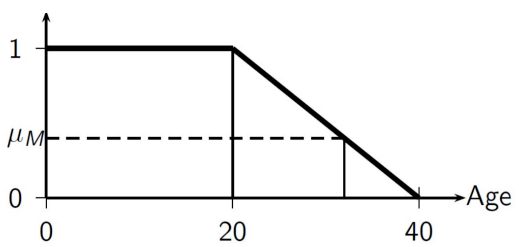
\includegraphics[width=0.5\columnwidth]{img/FS/young1}
\end{center}
A person is defined for sure "young" if he has an age of 20 or younger, and is for sure "not young" if over 40, everything in between has a varying degree of "youngness".\\

It doesn't have to be a linear function, other imprecise predicates could be modeled as other functions, such as a sigmoid.\\

Terms like "around" are modeled using different shapes (e.g., triangle, trapezoid, Gaussian, sigmoid, etc.). "Around 2" could be 1.8 or 2.3, it probably won't be 3 and it surely isn't 5.\\

\newpage

\subsubsection{Linguistic variables and linguistic values}

\textbf{Linguistic variables} represent \textbf{attributes} in fuzzy systems. They assume linguistic values.\\

\textbf{Linguistic values} usually \textbf{partition} the possible values of the linguistic variables subjectively (based on human intuition). All linguistic values have a \textbf{meaning}, not a precise numerical number.\\

\textbf{Example}: the linguistic variable is \textit{living area of a flat A}, and the values are \textit{tiny, small, medium, large, huge}
\begin{center}
	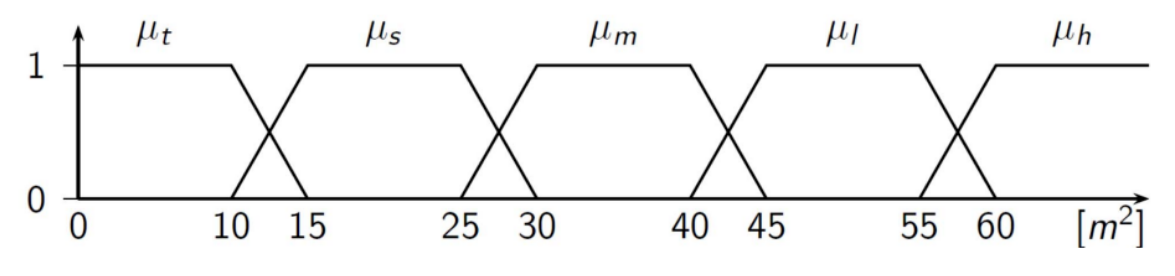
\includegraphics[width=0.9\columnwidth]{img/FS/living1}
\end{center}
Every $x \in A$ has $\mu (x) = [0,1]$ to each value.\\

\newpage

\subsubsection{Semantics of fuzzy sets}

What are we trying to model when we define a fuzzy set?\\

Fuzzy sets are relevant in 3 \textbf{types} of information-driven \textbf{tasks}: 
\begin{enumerate}
	\item Classification and data analysis
	\item Decision-making problems 
	\item Approximate reasoning
\end{enumerate}

These tasks exploit three \textbf{semantics of membership grades}: 
\begin{enumerate}
	\item Similarity 
	\item Preference 
	\item Possibility
\end{enumerate}

\paragraph{Degree of Similarity:} $\mu(u)$ is the degree of \textbf{proximity} of $u$ \textbf{from prototype} elements of $u$. Proximity between pieces of information is modeled. This view is used in: pattern classification, cluster analysis, regression. In fuzzy control similarity degrees are measured between current situation and prototypical ones.\\

\paragraph{Degree of Preference:} $\mu$ represents both a \textbf{set of} (more or less) \textbf{preferred objects} and \textbf{values} of a \textbf{decision variable} $X$, while $\mu (u)$ represents both \textbf{intensity of preference} in favor of object $u$ and \textbf{feasibility of selecting} $u$ as a value of $X$. Fuzzy sets represent criteria or \textbf{flexible constraints}. Used in: fuzzy optimization, decision analysis.\\

\paragraph{Degree of Possibility:} $\mu (u)$ can be viewed as degree of \textbf{possibility} that \textbf{parameter} $X$ has \textbf{value} $u$, given the only information "$X$ is $\mu$". It distinguishes plausible cases from less likely ones. Used in: expert systems, artificial intelligence.\\

\newpage

\subsubsection{Representation of Fuzzy sets}

\paragraph{Definition of a set:} By "set" we mean \textbf{every collection} made into a \textbf{whole} of definite, distinct objects of our intuition or of our thought.\\

Properties: 
\begin{itemize}
	\item $x \neq \{x\}$
	\item If $x \in X$ and $X \notin Y$, then $x \notin Y$
	\item The set of all subsets of $X$ is denoted as $2^X$
	\item $\emptyset$ is the empty set
\end{itemize}

\paragraph{Extension to a Fuzzy set:} A fuzzy set $\mu$ of $X \neq \emptyset$ is a \textbf{function} from the reference set $X$ to the unit interval, i.e., $$\mu: X \mapsto [0,1]$$

$\mathcal{F}(X)$ represents the \textbf{set of all fuzzy sets} of $X$, i.e.
$$ \mathcal{F}(X) := \{\mu | \mu X \mapsto [0,1] \} $$

\paragraph{Vertical Representation:} Fuzzy sets are described by their \textbf{membership function} and assigning \textbf{degree of membership} $\mu (x)$ to each element $x \in X$.\\

\textbf{Example}: linguistic expression "approximately between $b$ and $c$": 
$$ \mu_{a,b,c,d} (x) = \begin{cases}
	\frac{x - a}{b - a} & \text{ if } a \leq x \leq b \\
	1 & \text{ if } b \leq x \leq c \\
	\frac{x - d}{c - d} & \text{ if } c \leq x \leq d \\
	0 & \text{ if } x < a \text{ or } x > d
\end{cases}$$

\newpage

\paragraph{Horizontal Representation:} For all membership degrees belonging to chosen subset of $[0,1]$, human expert lists \textbf{elements of $X$ that fulfill vague concept of fuzzy set with degree} $\geq \alpha$. That is the horizontal representation of fuzzy sets by their \textbf{$\alpha$-cuts}. Definition: let $\mu \in \mathcal{F}(X)$ and $\in [0,1]$ Then the sets
$$ [\mu]_\alpha = \{x \in X | \mu (x) \geq \alpha \} $$
$$ [\mu]_{\underline{\alpha}} = \{x \in X | \mu (x) > \alpha \}$$
are called the $\alpha$-cut and strict $\alpha$-cut of $\mu$.\\

For each value $\alpha$ of the unit interval, we consider the set of elements having a membership degree of at least $\alpha$ to the fuzzy set.\\

\textbf{Example}: let $\mu$ be a triangular function on $\mathbb{R}$
\begin{center}
	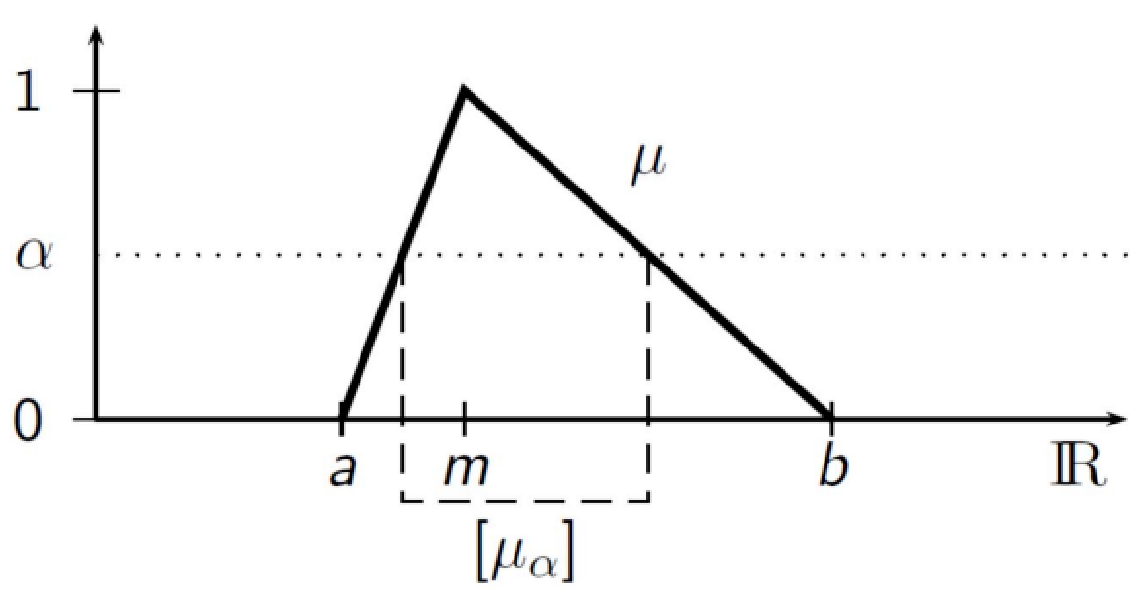
\includegraphics[width=0.45\columnwidth]{img/FS/hr1}
\end{center}
The $\alpha$-cut of $\mu$ can be constructed by: 
\begin{enumerate}
	\item Draw a horizontal line parallel to the $x$-axis through point $(0, \alpha)$
	\item project this section onto the $x$-axis
	$$ [\mu]_\alpha = \begin{cases}
		[a + \alpha(m-a), b - \alpha (b-m)] & \text{ if } 0 < \alpha \leq 1 \\
		\mathbb{R} & \text{ otherwise }
	\end{cases}$$
\end{enumerate}
Basically, it identifies the set of input values with a membership degree greater than $\alpha$.\\

\newpage

\textbf{Properties} of $\alpha$-cuts: 
\begin{itemize}
	\item \textbf{Any fuzzy set} can be \textbf{described} by \textbf{specifying its $\alpha$-cuts}. Let $\mu \in \mathcal{F} (X)$, $\alpha \in [0,1]$ and $\beta \in [0,1]$
	$$ [\mu]_0 = X$$
	$$ \alpha < \beta \implies [\mu]_\alpha \supseteq [\mu]_\beta $$
	\nn
	
	\item \textbf{Representation theorem}: let $\mu \in \mathcal{F} (X)$, then 
	$$ [\mu]_0 = \sup_{\alpha \in [0,1]} \left\{\min\left(\alpha, \mathcal{X}_{[\mu]_\alpha} (x)\right) \right\} $$
	$$ \text{where }\; \mathcal{X}_{[\mu]_\alpha} (x) = \begin{cases}
		1 & \text{ if } x \in [\mu]_\alpha \\
		0 & \text{ otherwise }
	\end{cases}$$
	Fuzzy sets can be obtained as upper envelope of its $\alpha$-cuts, simply draw $\alpha$-cuts parallel to horizontal axis in height of $\alpha$.\\
	In applications, it is recommended to select finite subset $L \subseteq [0,1]$ of relevant degrees of membership. They must be semantically distinguishable, fix level of fuzzy sets to characterize only for these levels.\\
\end{itemize}

This \textbf{representation} of fuzzy sets is \textbf{used in computers}. For example, suppose $X = [0, 15]$, an expert choose $L = \{0, 0.25, 0.5, 0.75, 1\}$ and $\alpha$-cuts:
\begin{itemize}
	\item $A_0 = [0,15]$
	\item $A_{0.25} = [3,15]$
	\item $A_{0.5} = [4,6] \cup [7,15]$
	\item $A_{0.75} = [4.5,5.5] \cup [7, 15]$
	\item $A_{} = \{5\} \cup [7,15]$
\end{itemize}
\begin{center}
	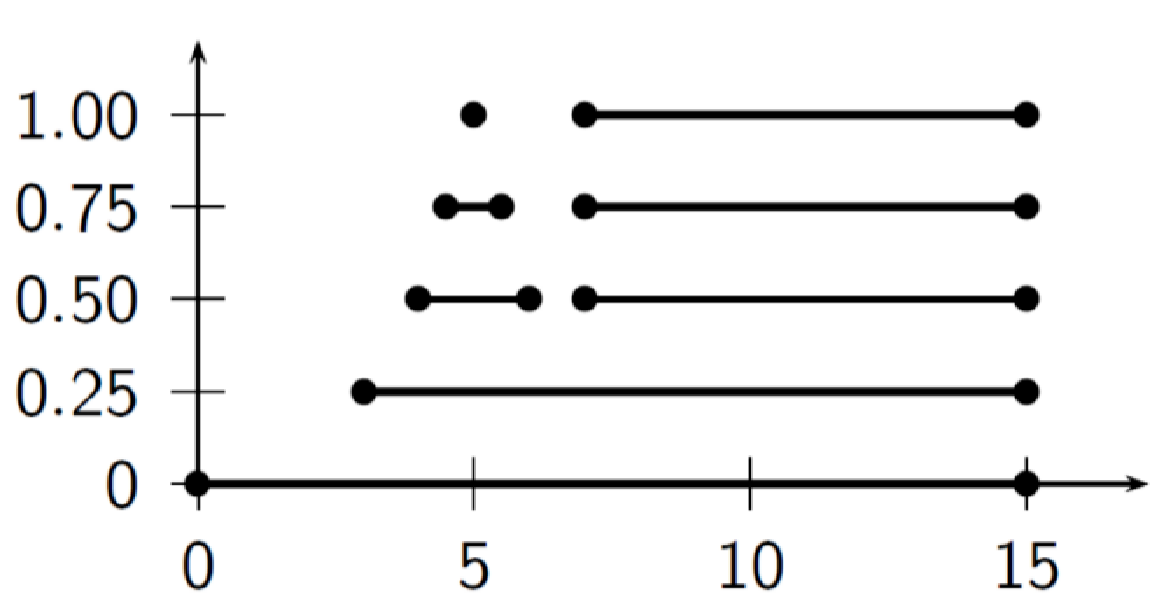
\includegraphics[width=0.55\columnwidth]{img/FS/hr2}
\end{center}

\newpage

We can see that $\mu_A$ is obtained as upper enveloper of the family $A$ of sets
\begin{center}
	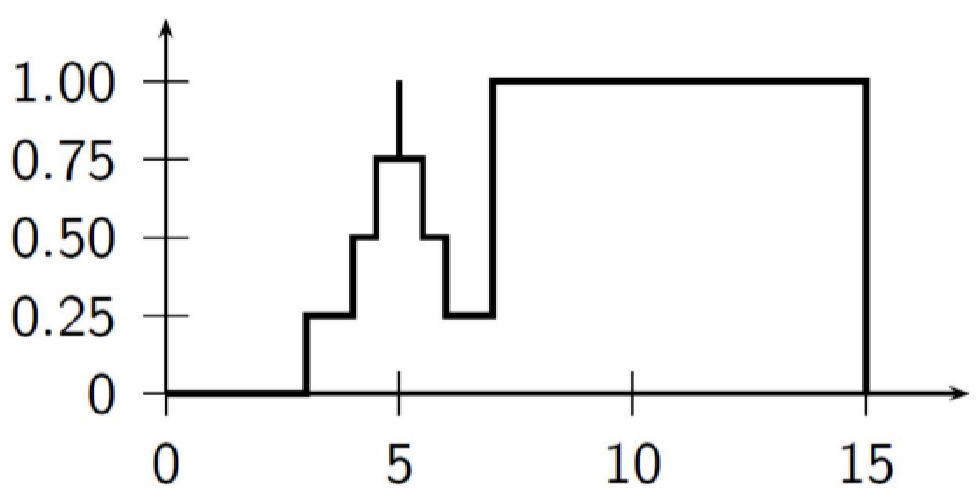
\includegraphics[width=0.55\columnwidth]{img/FS/hr3}
\end{center}
As stated before, this representation is \textbf{easier to process in computers} (it's basically a discrete quantization). Also, the domain of the $x$-axis is usually discretized as well.\\

Discretize the degrees of membership and obtain an approximation of the original fuzzy set. Depending on the considered problem, it must be chosen how fine the discretization should be, there are no general rules.\\
The fuzzy sets are usually determined heuristically or can only be specified roughly.\\

Fuzzy sets are usually stored inside a computer as a chain of linear lists, for each $\alpha$-level, $\alpha \neq 0$.
\begin{center}
	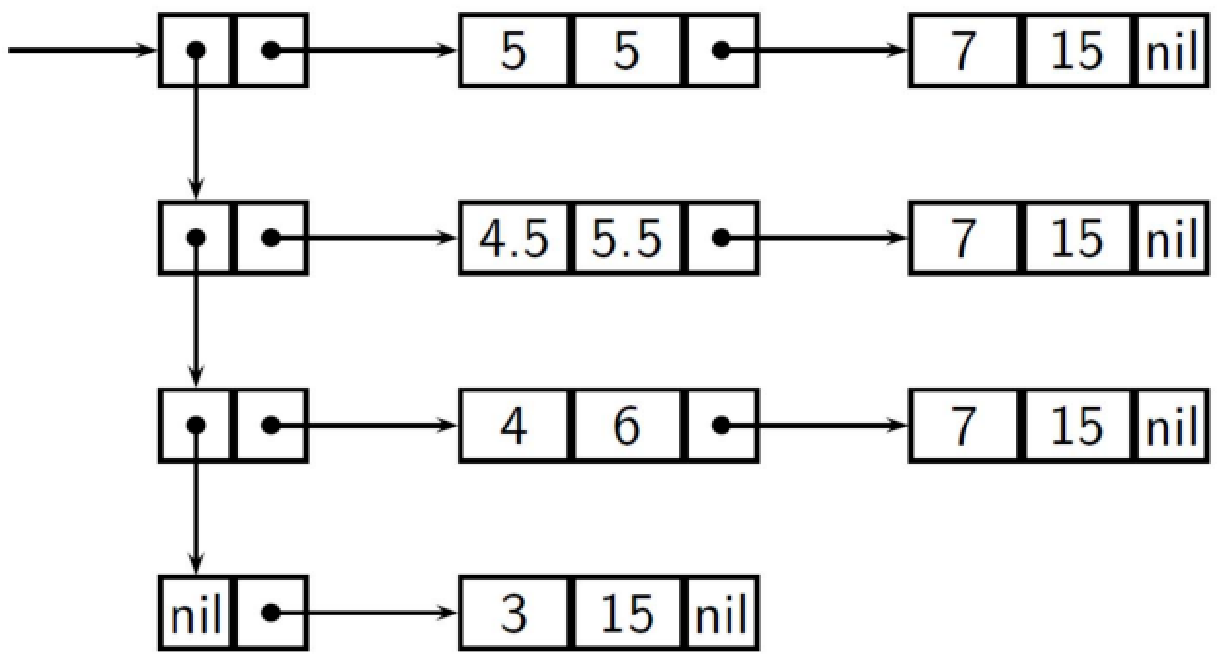
\includegraphics[width=0.7\columnwidth]{img/FS/hr4}
\end{center}
A finite union of closed intervals is stored by their bounds.\\

This data structure is appropriate for arithmetic operators.\\

\newpage

\subsubsection{Support, Core and Height}

\paragraph{Support:} The \textbf{support} $S(\mu)$ of a fuzzy set $\mu \in \mathcal{F}(X)$ is the crisp \textbf{set} that contains \textbf{all elements} of $X$ that have \textbf{nonzero membership} 
$$ S(\mu) = [\mu]_{\underline{0}} = \{x \in X | \mu (x) > 0 \} $$
Basically, the area of the fuzzy set for which the degree of membership is more than zero.\\ \nn

\paragraph{Core:} The \textbf{core} $C(\mu)$ of a fuzzy set $\mu \in \mathcal{F} (X)$ is the crisp \textbf{set} that contains \textbf{all elements} of $X$ that have \textbf{membership of one}
$$ C(\mu) = [\mu]_1 = \{x \in X | \mu(x) = 1 \} $$
All the elements for which I'm sure the linguistic attribute is applicable.\\ \nn

\paragraph{Height:} The \textbf{height} $h(\mu)$ of a fuzzy set $u \in \mathcal{F} (X)$ is the \textbf{largest membership grade} obtained by any element in that set 
$$ h(\mu) = \sup_{x \in X} \{\mu (x)\} $$
A fuzzy set is called \textbf{normal} iff $h (\mu) = 1$, it is called \textbf{subnormal} iff $h(\mu) < 1$.\\

\newpage

\subsubsection{Convex fuzzy sets}
Let $X$ be a vector space. A fuzzy set $\mu \in \mathcal{F} (X)$ is called \textbf{fuzzy convex} if its $\alpha$-cuts are convex for all $\alpha \in (0,1]$.\\

The \textbf{membership function} of a convex fuzzy set is \textbf{not a convex function}.\\

Classical definition: the membership functions are actually \textbf{concave}.\\

\subsubsection{Fuzzy Numbers}
A fuzzy set $\mu$ is a \textbf{fuzzy number} if and only if $\mu$ is \textbf{normal} and $[\mu]_\alpha$ is \textbf{bounded}, \textbf{close}, and \textbf{convex} $\forall \alpha \in (0, 1]$. For example, the term \textit{approximately} $x_0$ is described by a parameterized class of membership functions.
$$ 
\begin{cases}
	[1, 2] & \text{ if } \alpha \geq 0.5 \\
	[0.5 + \alpha, 2) & \text{ if } 0 > \alpha < 0.5 \\
	\mathbb{R} & \text{ if } \alpha = 0
\end{cases}
$$
\begin{center}
	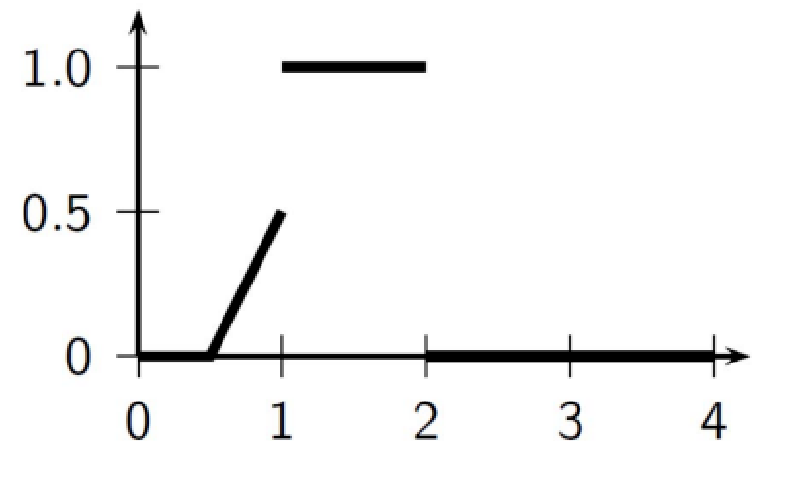
\includegraphics[width=0.4\columnwidth]{img/FS/numbers1}
\end{center}
Upper semi-continuous functions are often convenient in applications. In many applications the class of the functions and their exact parameters have a limited influence on the results. In other applications more precise membership degrees are needed. \\

\newpage

\subsection{Multi-Valued Logics}

The fuzzy concepts seen before referred to a single variable, but how do I compare/combine multiple variables? We need to define a multi-valued logic.\\

\subsubsection{Usual logic concepts}

\paragraph{Set operators:} They are defined by using \textbf{traditional logics operators}. Let $X$ be the universal set: 
\begin{itemize}
	\item $A \cap B = \{x \in X | x \in A \vee x \in B\}$
	\item $A \cup B = \{x \in X | x \in A \wedge x \in B\}$
	\item $A^c = \{x \in X | x \notin A\} = \{x \in X | \neg (x \in A)\}$
	\item $A \subseteq B$ if and only if $(x \in A) \implies (x \in B)$ for every $x \in X$
\end{itemize}

\paragraph{Classical logic:} Considers value which are either \textit{true} or \textit{false}. Propositional logic handles combination of logical variables. The key idea is to express $n$-ary logic functions with logic primitives. \\

A set of logic primitives is \textbf{complete} if \textit{any logic function} can be composed by a finite number of these primitives, e.g.
$$ \wedge, \vee, \neg, NOR, NAND, | $$

\paragraph{Inference rules:} When a variable represented by a logical formula is \textbf{true} for all possible truth values it is called \textbf{tautology}. Instead, when it is \textbf{false} for all possible truth values it is called \textbf{contradiction}. \\

Various forms of tautologies exist to perform deductive inference, and are called \textbf{inference rules}:
\begin{itemize}[label*=]
	\item $(a \wedge (a \rightarrow b)) \rightarrow b$ (modus ponens)
	\item $(\neg b \wedge (a \rightarrow b)) \rightarrow \neg a$ (modus tollens)
	\item $((a \rightarrow b) \wedge (b \rightarrow c)) \rightarrow (a \rightarrow c)$ (hypothetical syllogism)
\end{itemize}

\paragraph{Boolean algebra:} The propositional logic based on finite set of logic variables is isomorphic to finite set theory. Both of these systems are isomorphic to a finite Boolean algebra. %Definition: a Boolean algebra on a set $B$ is defined as quadruple $\mathcal{B} = (B, +, \cdot , \overline{ })$, where $B$ has at least two elements $0$ and $1$, $+$ and $\cdot$ are binary operators on $B$, and $\overline{ }$ is a unary operator on $B$ for the which the following properties hold:

\newpage

\subsubsection{$n$-valued logics}

2-valued logic can be extended to a 3-valued logic in several ways, for example: 
\begin{center}
	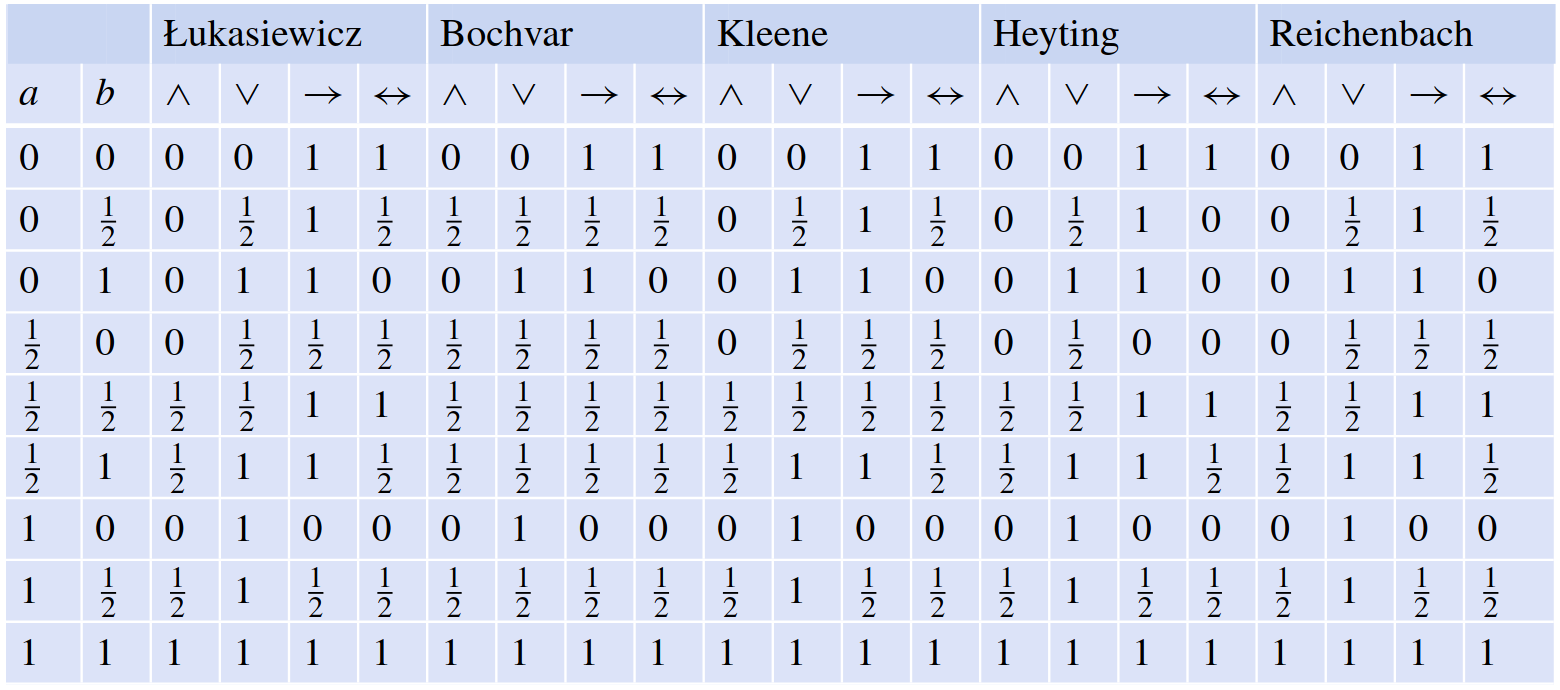
\includegraphics[width=0.95\columnwidth]{img/FS/nlogic}
\end{center}
These examples allow for an indeterminate value $\sfrac{1}{2}$. There is no standard interpretation of the truth degrees.\\

Various \textbf{$n$-valued logics} exists. The idea is to \textbf{uniformly divide} the range $[0,1]$ into $n$ \textbf{truth values}, which can be interpreted as \textbf{degrees of truth}. Definition: the set $T_n$ of truth values of an $n$-valued logic is defined as
$$ T_n = {0 = \frac{0}{n-1}, \frac{1}{n-1}, \frac{2}{n-1}, \, \dots \, , \frac{n-2}{n-1}, \frac{n-1}{n-1} = 1} $$

\paragraph{Primitives in $n$-valued logic:} Generalization of \l{L}ukasiewicz three valued logic. It uses truth values in $T_n$ and defines primitives as follows
$$ \neg a = 1 - a $$
$$ a \wedge b = \min (a,b) $$
$$ a \vee b = \max(a,b) $$
$$ a \rightarrow b = \min(1, 1 + b - a) $$
$$ a \leftrightarrow b = 1 - |a - b| $$

This $n$-valued logic is denoted by $L_n$. The sequence $(L_2, L_3, \, \dots \, , L_{\infty})$ contains the classical two-valued logic $L_2$ and an infinite-valued logic $L_{\infty}$ (rational countable values $T_{\infty}$). The infinite-valued logic $L_1$ is the logic with all real numbers in $[0, 1]$ ($1=$ cardinality of continuum).

\newpage

\subsubsection{Fuzzy set theory}

\textit{What does a fuzzy set represent?} A \textbf{logic with values in the range} $[0,1]$. \\

Consider the \textit{fuzzy proposition} $A$ ("approximately two" in the example) on $\mathbb{R}$, fuzzy logic offers means to construct such imprecise sentences

\begin{center}
	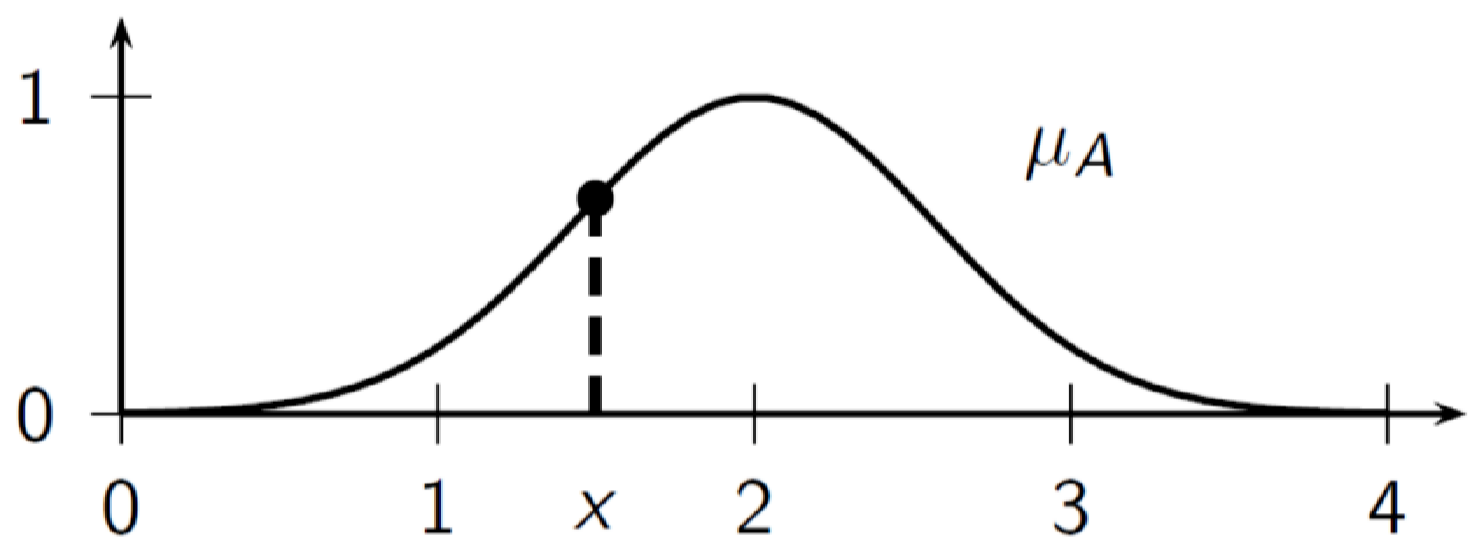
\includegraphics[width=0.6\columnwidth]{img/FS/appr2}
\end{center}

$A$ is \textbf{defined} by a \textbf{membership function} $\mu_A$, i.e., truth values $\forall x \in \mathbb{R}$; let $x \in \mathbb{R}$ be a \textbf{subject/observation}, $\mu_A (x)$ is the \textbf{degree of truth} that $x$ is $A$.\\

\paragraph{Standard fuzzy set operators:} We define the following \textbf{algebraic operators} on $\mathcal{F} (X)$ 
\begin{itemize}
	\item $(\mu \wedge \mu') := \min \{\mu(x), \mu' (x)\}$ \textbf{intersection} (AND)
	\item $(\mu \vee \mu') := \max \{\mu(x), \mu' (x)\}$ \textbf{union} (OR)
	\item $\neg \mu := 1 - \mu (x)$ \textbf{complement} (NOT)
\end{itemize}
$\mu$ is subset of $\mu'$ if and only if $\mu \leq \mu'$.\\

\begin{center}
	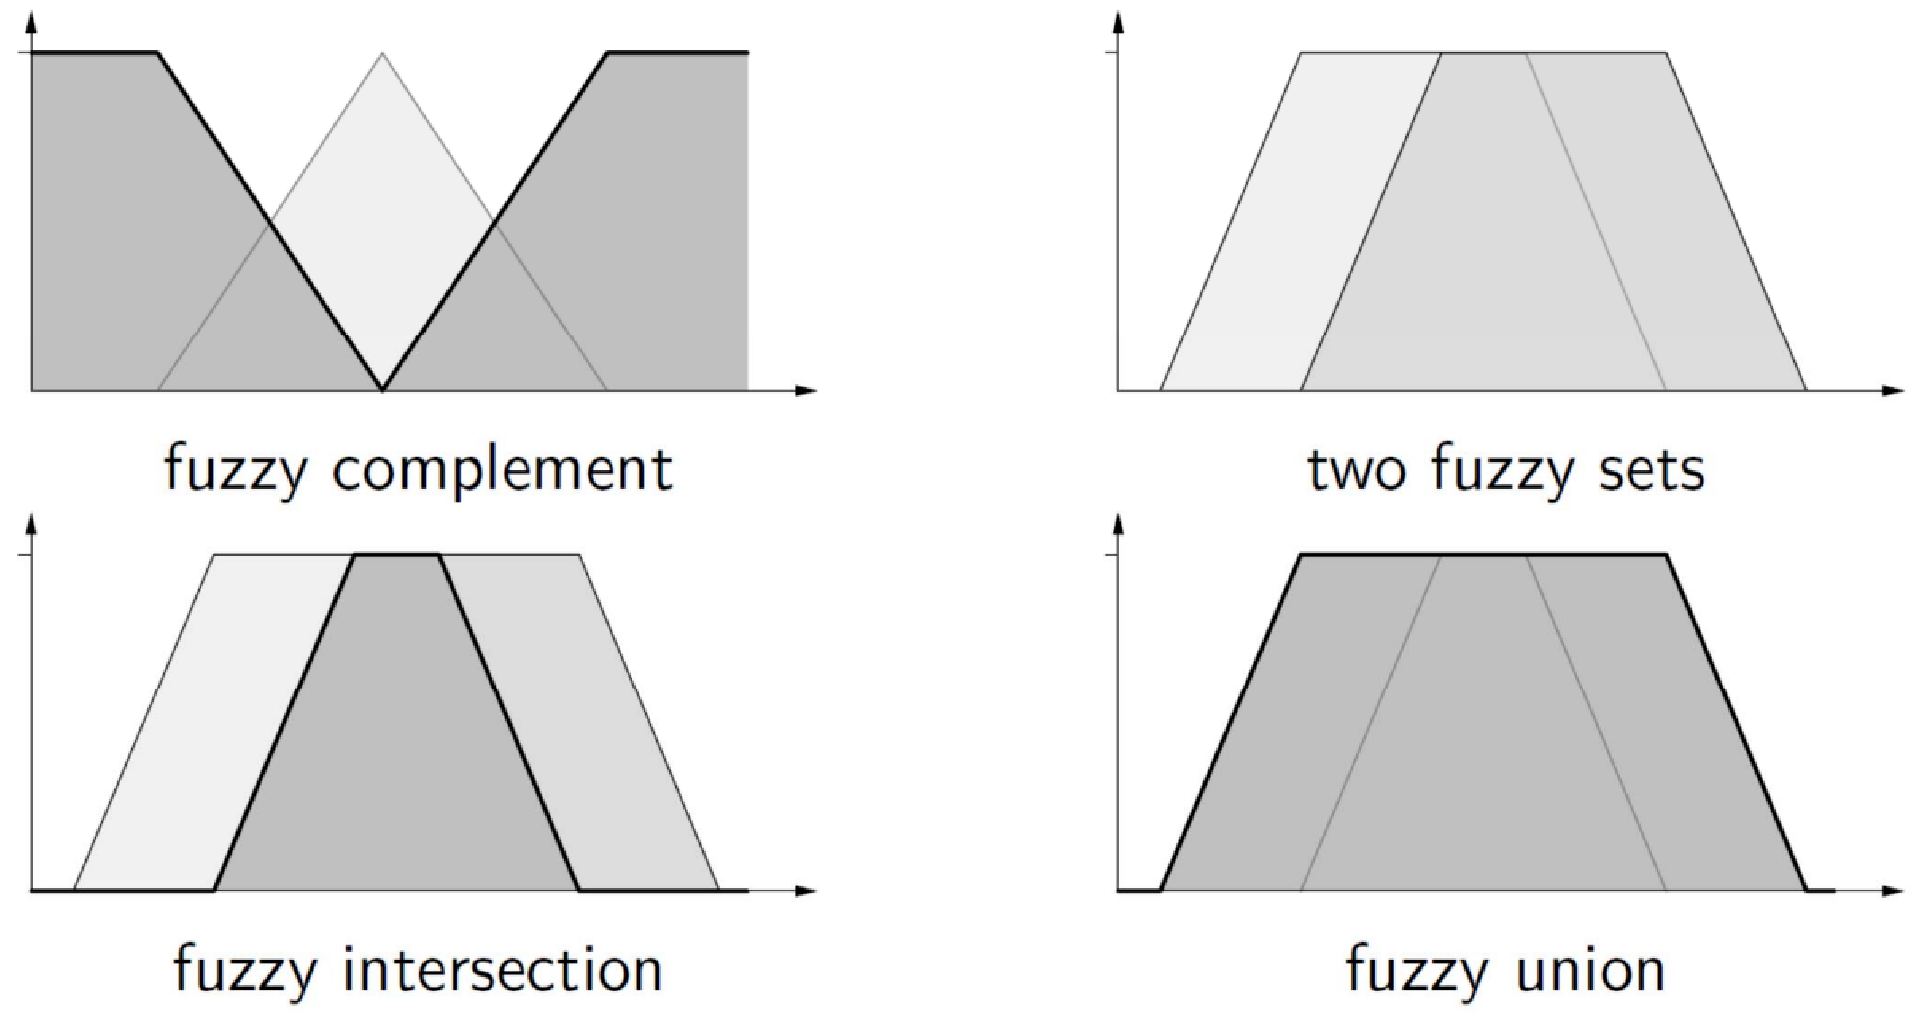
\includegraphics[width=0.8\columnwidth]{img/FS/fop1}
\end{center}

\textbf{Theorem:} $\mathcal{F} (X), \wedge, \vee, \neg)$ is a complete distributive lattice but not a Boolean algebra.

\newpage

\paragraph{Fuzzy set complement/negation:} Let $X$ be a given set and $\mu \in \mathcal{F} (X)$. Then the complement $\overline{\mu}$ can be defined pointwise by $\overline{\mu} (x) := \sim (\mu (x))$, where $\sim: [0, 1] \mapsto [0,1]$ satisfies the conditions
$$ \sim (0) = 1 \;\;\;\;\;\;\; \sim (1) = 0 $$
and for $x,y \in [0,1]$, $x \leq y \implies \sim x \geq \sim y$ ($\sim$ is non-increasing).\\

A negation is called \textbf{strict} if it is also strictly decreasing (as above but $<$ instead of $\leq$) and continuous. A strict negation is said to be \textbf{strong} if it is \textbf{involutive} ($\sim \sim x = x$, $\forall x \in [0,1]$), too.\\

\textbf{Families of negation}: 
\begin{itemize}
	\item Standard negation
	$$ \sim x = 1 - x $$
	\item Threshold negation
	$$ \neg_\theta x = \begin{cases}
		1 & \text{ if } x \leq \theta \\
		0 & \text{ otherwise }
	\end{cases}$$
	\item Cosine negation: 
	$$ \sim x = \frac{1}{2} (1 + \cos (\pi x)) $$
	\item Sugeno negation: 
	$$ \sim x = \frac{1 - x}{1 + \lambda x}, \;\;\;\;\; \lambda \succ 1$$
	\item Yager negation
	$$ \sim x = (1 - x^\lambda)^{\frac{1}{\lambda}} $$
\end{itemize}

\begin{center}
	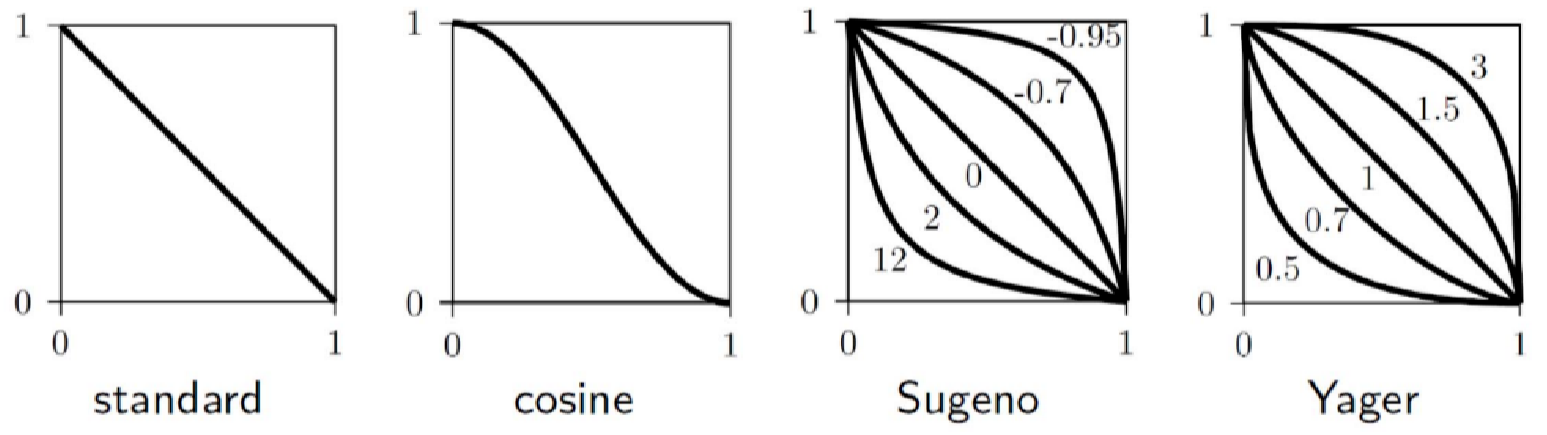
\includegraphics[width=0.95\columnwidth]{img/FS/famneg}
\end{center}

No need to remember everything, just note that there can be \textbf{different types of negation}.\\

\newpage

\paragraph{Fuzzy set intersection and union:} Classical set intersection represents logical conjunction. Classical set union represents logical disjunction. \\

Generalization from $\{0,1\}$ to $[0,1]$: Let $A, B$ be fuzzy subsets of $X$, i.e., $A,B \in \mathcal{F} (X)$. Their intersection and union can be defined pointwise using: 
\begin{itemize}[label*=]
	\item T-norm: $(A \cap B) (x) = \top (A(x), B(x))$ where $\top : [0,1]^2 \mapsto [0,1]$
	\item T-Conorm: $(A \cup B) (x) = \bot (A(x), B(x))$ where $\bot : [0,1]^2 \mapsto [0,1]$
\end{itemize}

$\top$ and $\bot$ are called \textbf{triangular norm} and \textbf{triangular conorm}, they take 2 values and give back \textit{something}. For all values they respect identity law, commutativity, associativity and monotonicity. \\

\paragraph{Minimum and Maximum:} Min is the greatest t-norm and max is the weakest t-conorm
$$ \top_{\min} = \min (x, y) \;\;\;\;\;\; \bot_{\max} (x,y) = \max (x, y)$$
So $\top (x,y) \leq \min (x,y)$ and $\bot (x,y) \geq \max (x,y)$ for ant $\top$ and $\bot$.\\

We can choose other function as t-norm or t-conorm which are less \textit{harsh}, but $\top_{\min}$ and $\bot_{\max}$ can be easily processed numerically and visually.\\

\paragraph{Product and Probabilistic Sum:} We can use other functions such as product and sum: 
$$ \top_{\text{prod}} (x,y) = x \cdot y \;\;\;\;\;\; \bot_{\text{sum}} (x,y) = x + y - x \cdot y $$
The use of product and its dual has nothing to do with probability theory.\\

\vfill 

And there are a bunch of other T-norms and conorms which I won't describe right now, but I will name: \textbf{\l{L}ukasiewicz T-Norm and T-Conorm, Nilpotent minimum and maximum, drastic product and sum}.

\newpage

\textbf{Examples} of fuzzy \textbf{intersections:}
\begin{center}
	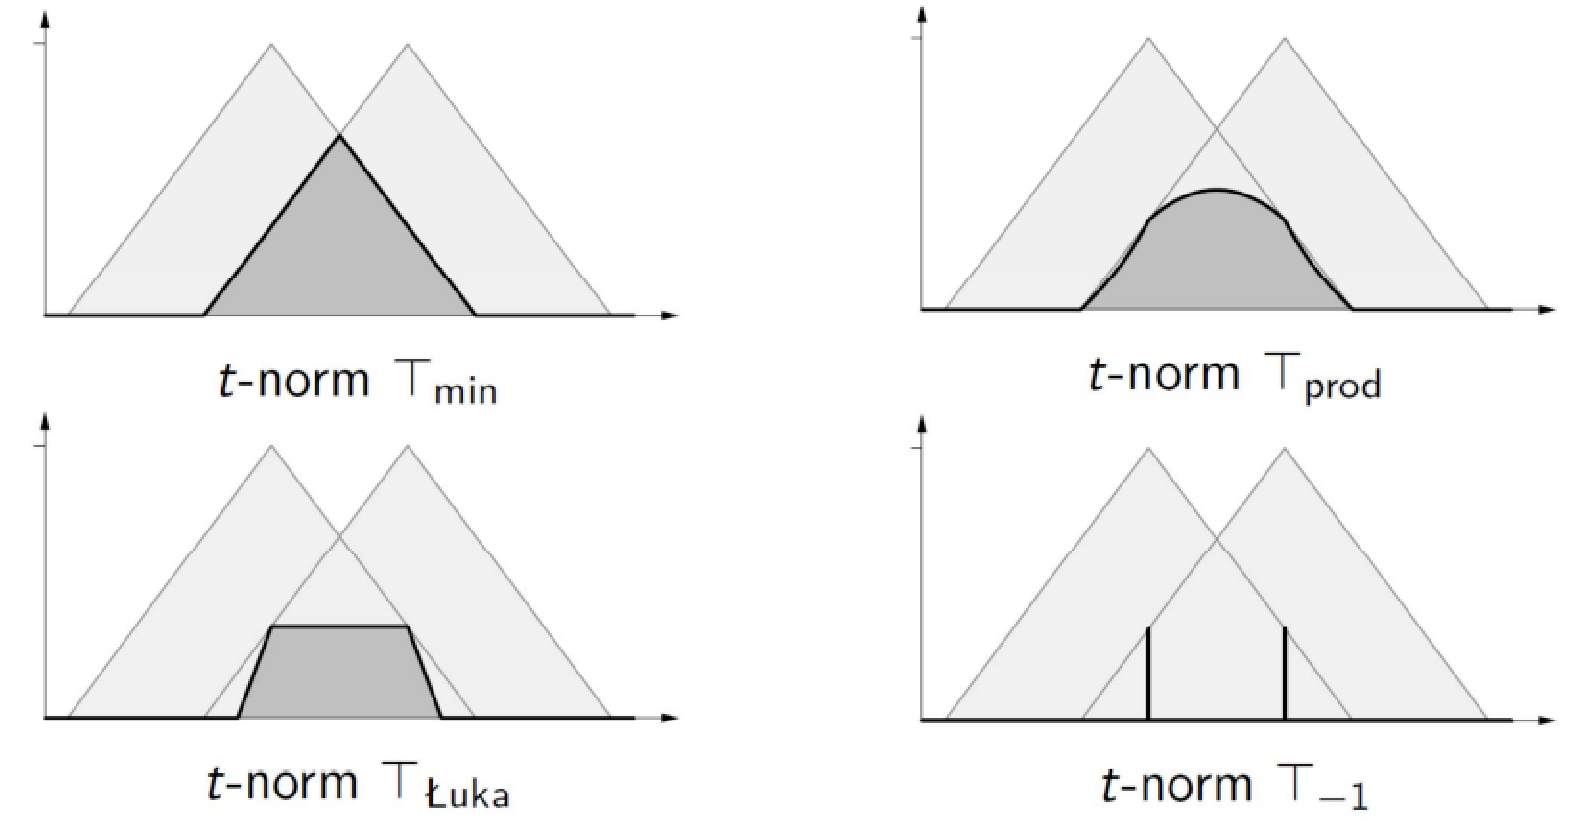
\includegraphics[width=0.9\columnwidth]{img/FS/fint}
\end{center}

\textbf{Examples} of fuzzy \textbf{unions:}
\begin{center}
	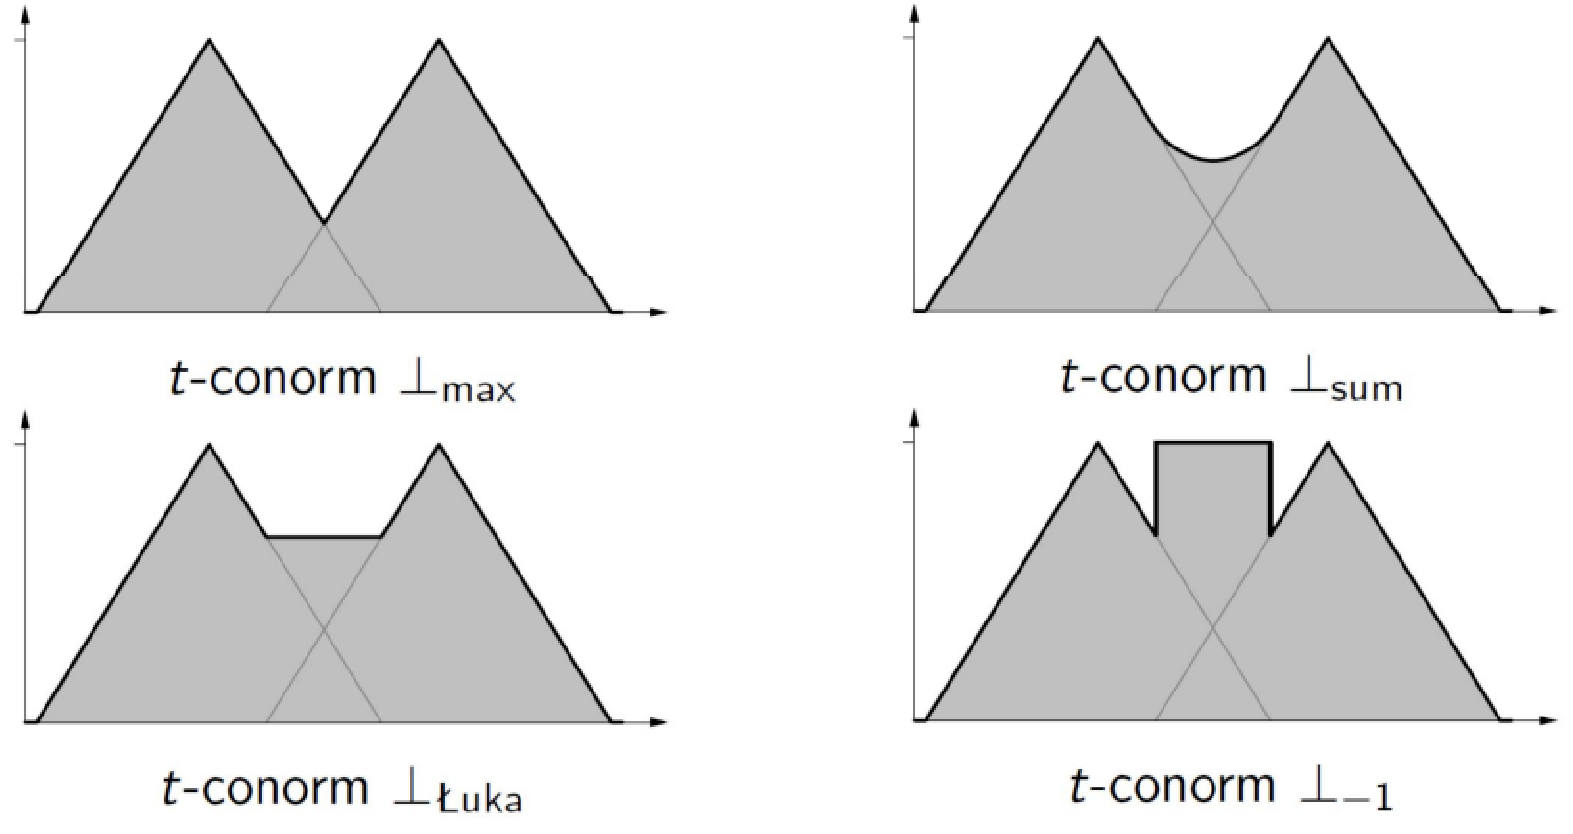
\includegraphics[width=0.9\columnwidth]{img/FS/funion}
\end{center}

There are different intersection/union areas.\\

\newpage

\subsubsection{Fuzzy Implication}

Regarding the \textbf{implication} (if $x$ belongs to $A$ then it belongs to $B$), there are different ways in which fuzzy implications can be defined.\\

One way of defining $I$ is to use $\forall a,b \in \{0,1\}$
$$ I (a,b) = \neg a \wedge b $$

In fuzzy logic, disjunction and negation are t-conorm and fuzzy complement, respectively, thus $\forall a,b \in [0,1]$:
$$ I(a,b) = \bot (\sim a,b) $$

Another way in classical logic is $\forall a,b \in \{0,1\}$
$$ I (a,b) = \max \{x \in \{0,1\} | a \wedge x \leq b \} $$

In fuzzy logic, conjunction represents t-norm, thus $\forall a,b \in [0,1]$
$$ I(a,b) = \sup \{x \in [0,1] | \top (a,x) \leq b \} $$

Classical definitions are equal, fuzzy extensions are not: law of absorption of negation does not hold in fuzzy logic.\\

\newpage

There are \textbf{different ways of handling implications} in \textbf{fuzzy logic}, depending on how the implication is defined:
\begin{itemize}
	\item \textbf{$S$-Implications:} implications based on $I(a,b) = \bot (\sim a,b)$. The symbol $S$ is often used to denote t-conorms.\\
	
	\item \textbf{$R$-Implications:} implications based on $I(a, b) = \sup \{x \in [0, 1]| \top (a, x) \leq b\}$ are called $R$-implication. The symbol $R$ represents close connection to residuated semigroup (whatever this means).\\
	
	\item \textbf{$QL$-implications:} implications based on $\bot (\sim a, \top(a, b))$ are called $QL$-implications, where $QL$ stands for quantum logic.\\
\end{itemize}

\paragraph{Conclusions:} All $I$ come from generalizations of the classical implication. They collapse to the classical implication when truth values are $0$ or $1$. \\

\textit{Which fuzzy implication should be used for calculating the fuzzy relation $R$?} Since the meaning of $I$ is not unique, we must resolve this question. Meaningful criteria are needed, it depends on the situation. \\

\newpage

%End FS L1, app 103

\newpage

\subsection{Theory of Fuzzy Logic}

\subsubsection{The Extension principle}

How do we \textbf{extend operations} to the concept of \textbf{fuzzy sets}.\\

How do we extend functions \textbf{defined on sets to} functions \textbf{defined on fuzzy sets}?
$$ \text{from } \; \phi : X^n \rightarrow Y \; \text{ to } \; \hat \phi : \mathcal{F} (x)^n \rightarrow \mathcal{F} (Y) $$

Let $\mu \in \mathcal{F} (\mathbb{R})$ be a fuzzy set of the \textit{imprecise concept} "about 2", then the degree of membership $\mu (2.2)$ can be seen as truth value of the statement "2.2 is about equal to 2".\\

Any \textit{triangular norm} (t-norm) $\top$: can represent \textbf{conjunction}.\\
Any \textit{triangular co-norm} (t-conorm) $\bot$: can represent \textbf{disjunction}.\\
However, now only $\top_{\min}$ and $\bot_{\max}$ will be used (conjunction of two statements becomes taking the minimum, maximum for the disjunction).\\

Let $\mathcal{P}$ be a \textbf{set of imprecise statements} that can be combined by the operators "\textit{and}" and "\textit{or}", define the \textbf{function} $truth$:
\begin{itemize}
	\item $truth: \mathcal{P} \rightarrow [0,1]$ assigns truth value truth$(a)$ to every $a \in \mathcal{P}$
	\item $truth(a) = 0$ means $a$ is definitely false
	\item $truth(a) = 1$ means $a$ is definitely true
	\item If $0 < truth(a) < 1$ then only gradual truth of statement $a$ 
\end{itemize}

\textbf{Combination} of \textbf{two statements}: 
\begin{itemize}
	\item $truth (a \aand b) = truth(a \wedge b) = \min\{truth(a), truth(b) \}$
	\item $truth (a \oor b) = truth(a \vee b) = \max\{truth(a), truth(b) \}$
\end{itemize}
The $\top$ and $\bot$ for this case, since there's no boolean logic.\\

Extended for an \textbf{infinite number of statements} $a_i$, $i \in I$:
\begin{itemize}
	\item $truth(\forall i \in I: a_i) = \inf \{truth (a_i) | i \in I \}$
	\item $truth(\exists i \in I: a_i) = \sup \{truth (a_i) | i \in I \}$
\end{itemize}
Respectively, the minimum degree of truth satisfied by all and the maximum degree of at least one statement.\\

\newpage

This concept helps to extend $\phi: X^n \rightarrow Y$ to $\hat \phi : \mathcal{F}(X)^n \rightarrow \mathcal{F}(Y)$
\begin{itemize}[label*=]
	\item Crisp tuple $(x_1, \, \dots \, , x_n)$ is mapped to the crisp value $\phi (x_1, \, \dots \, , x_n)$.\\
	
	\item Imprecise descriptions $(\mu_1 , \, \dots \, , \mu_n)$ of $(x_1, \, \dots \, , x_n)$ are mapped to fuzzy value $\hat \phi (\mu_1, \, \dots \, , \mu_n)$.\\
\end{itemize}

\paragraph{Example:} How to extend the addition? With the sum extended to sets
$$ +: 2^{\mathbb{R}} \times 2^{\mathbb{R}} \rightarrow 2^{\mathbb{R}}, \;\;\;\;\; (A,B) \mapsto A + B $$
$$ = \{y | (\exists a) (\exists b) (y = a + b) \wedge (a \in A) \wedge (b \in B) \} $$
(still a sum, just with elements from the sets).\\

This can be \textbf{extended to fuzzy sets}: 
$$ +: \mathcal{F} (\mathbb{R}) \times \mathcal{F} (\mathbb{R}) \rightarrow \mathcal{F} (\mathbb{R}), \;\;\;\;\; (\mu_1, \mu_2) \mapsto \mu_1 \oplus \mu_2$$

$$ truth (y \in \mu_1 \oplus \mu_2) $$
$$ = truth ((\exists a) (\exists b): (y = a + b) \wedge (a \in \mu_1) \wedge (b \in \mu_2)) $$

Up until now it's the same as before. $\exists$ means taking the $\sup$ (as seen earlier), so:
$$ = \sup_{a,b} \{truth (y = a + b) \wedge truth (a \in \mu_1) \wedge truth (b \in \mu_2)\}$$
$$ = \sup_{a,b: y=a+b} \{\min (\mu_1(a), \mu_2(b))\}$$

The greatest $a$ and $b$ such that $y = a+b$ and we consider the minimum of the fuzzy memberships of said $a$ and $b$.\\

\newpage

\paragraph{In general:} A function $\phi: X^n \rightarrow Y$ can be extended to classic sets $\hat \phi: [2^X]^n \rightarrow 2^Y$ with 
$$ \hat \phi (A_1, \, \dots \, , A_n) = \{y \in Y | \exists (x_1 \, \dots \, , x_n) \in A_1 \times \, \dots \, \times A_n : \phi (x_1, \, \dots \, x_n) = y\} $$

And then we can \textbf{generalize to fuzzy sets}:
$$ \hat \phi: [\mathcal{F} (X)]^n \rightarrow \mathcal{F} (Y) $$
with 
$$ \hat \phi (A_1, \, \dots \, , A_n) = \sup \{ \min \{ \mu_1 (x_1), \, \dots \, , \mu_n (x_n) \} |$$ 
$$| (x_1, \, \dots \, , x_n) \in X^n \wedge \phi (x_1, \, \dots \, , x_n) = y \}$$

Assuming that sup $\emptyset = 0$.\\

The mapping of the fuzzy variable is the greatest values of the tuple belonging to $X^n$ such that the minimum of the fuzzy membership is greatest. \\

The minimum of the fuzzy sets should be the greatest, this is the extension principle.\\

\newpage

\subsubsection{Relevant Fuzzy sets}

We'll give particular relevance to fuzzy sets \textbf{defined on} $\mathbb{R}$, with membership function such as
$$ \mu : \mathbb{R} \rightarrow [0,1] $$

These clearly have a \textit{quantitative meaning} and may essentially characterize the \textbf{states of fuzzy variables}. They play an important role in many applications such as fuzzy control, decision-making, approximate reasoning, etc.\\

\textbf{Some relevant classes} $\mathcal{F} (\mathbb{R})$ (set of fuzzy sets) of fuzzy sets $\mu$ (a single fuzzy set) on $\mathbb{R}$ are defined as: 
\begin{itemize}
	\item \textbf{Normal Fuzzy Set:}
	$$ \mathcal{F}_N (\mathbb{R}) := \left\{\mu \in \mathcal{F} (\mathbb{R}) | \exists x \in \mathbb{R}: \mu (x) = 1 \right\} $$
	There's at least an element inside the fuzzy set equal to 1. The maximum membership has to be assigned to \textit{some value}. These make sense in the case of fuzzy numbers ("about 2" will have membership $=1$ for the value 2).\\
	
	\item \textbf{Upper Semi-continuous Fuzzy Set:}
	$$ \mathcal{F}_C (\mathbb{R}) := \left\{\mu \in \mathcal{F}_N (\mathbb{R}) | \forall \alpha \in (0,1] : [\mu]_\alpha \text{ is compact } \right\} $$
	Can be described by an upper semi-continuous function. Not continuous, but at the discontinuity point it includes the upper point, it's \textit{almost continuous}.\\
	
	\item \textbf{Fuzzy Intervals:}
	$$ \mathcal{F}_I (\mathbb{R}) := \left\{\mu \in \mathcal{F}_N (\mathbb{R}) | \forall a,b,c \in \mathbb{R} : c \in [a,b] \right\}$$
	$$ \implies \mu(c) \geq \min\{\mu(a), \mu(b)\} $$
	Membership drops gradually outside a certain interval. Their core is a classical interval, the edges (support) are a slope towards zero.\\
\end{itemize}

\newpage

\subsubsection{Quantitative Fuzzy Variables}

The concept of a fuzzy number plays a fundamental role in formulating \textbf{quantitative fuzzy variables}. These are variables whose \textbf{states are fuzzy numbers}.\\

When the fuzzy quantities \textbf{represent linguistic concepts}, e.g., very small, medium, large etc., then the fuzzy variables are called \textbf{linguistic variables}. Each linguistic variable is \textbf{defined in terms of base variable} which is a variable in the classical sense, e.g., temperature, pressure, age.\\

Linguistic terms \textbf{representing approximate values} of \textbf{base variable} are \textbf{captured by} appropriate \textbf{fuzzy numbers}.\\

Each linguistic variable is \textbf{defined by a quintuple} $(v, T, X, g, m)$ where:
\begin{itemize}
	\item $v$ is the \textbf{name} of the variable
	\item $T$ is the \textbf{set of linguistic terms} of $v$
	\item $X \subseteq \mathbb{R}$ is the \textbf{base variable}
	\item $g$ is the \textbf{syntactic rule} (grammar) for generating linguistic terms
	\item $m$ is the \textbf{semantic rule} that assigns meaning $m(t)$ to every $t \in T$, i.e., $m: T \rightarrow \mathcal{F} (X)$
\end{itemize}

To deal with linguistic variables we need to consider not only set-theoretic operations but also arithmetic operations on fuzzy numbers (i.e., interval arithmetic; something that has a quantitative meaning, e.g., how do we define the double of a fuzzy value? How do we get statistics?).\\

\vfill 

Examples MIA. \\

\newpage

\subsubsection{Efficient Operations}
How do we define \textbf{arithmetic operations} for \textbf{calculating with} $\fr$? In general operations on fuzzy set are \textbf{more complex}.\\

Using \textbf{extension principle} for sum $\mu \oplus \mu'$, product $\mu \odot \mu'$ and reciprocal value $rec(\mu)$ if arbitrary fuzzy sets $\mu, \mu' \in \fr$
$$ (\mu \oplus \mu') (t) = \sup \{\min \{\mu(x_1), \mu'(x_2)\} | x_1, x_2 \in \mathbb{R}, x_1 + x_2 = t\}$$
$$ (\mu \odot \mu') (t) = \sup \{\min \{\mu(x_1), \mu'(x_2)\} | x_1, x_2 \in \mathbb{R}, x_1 \cdot x_2 = t\}$$
$$ rec (\mu) (t) = \sup \left\{\mu(x) | x \in \mathbb{R} \setminus \{0\}, \frac{1}{x} = t \right\} $$

It's desirable to \textbf{reduce fuzzy arithmetic to ordinary set arithmetic}. Then, we apply elementary operations of interval arithmetic.\\

We have to define the set representation.\\

\paragraph{Definition:} A family $(A_\alpha)_{\alpha \in (0,1)}$ of sets is called \textbf{set representation} of $\mu \in \fnr$ if 
\begin{itemize}
	\item $0 < \alpha < \beta < 1 \implies A_\alpha \subseteq A_\beta \subseteq \mathbb{R}$ and
	\item $\mu (t) = \sup \{ \alpha \in [0,1] | t \in A_\alpha \}$
\end{itemize}
holds where $\sup \emptyset = 0$. If the $\alpha$-cuts represent the fuzzy membership we can do the operation on the fuzzy interval.\\

\paragraph{Theorem:} Let $\mu \in \fnr$. The family $(A_\alpha)_{\alpha \in (0,1)}$ is a set representation of $\mu$ if and only if 
$$ [\mu]_{\underline{\alpha}} = \left\{t \in \mathbb{R} | \mu(t) > \alpha \right\} \subseteq A_\alpha \subseteq \left\{t \in \mathbb{R} | \mu(t) \geq \alpha\right\} = [\mu]_\alpha$$
is valid for all $\alpha \in (0,1)$.\\

Let $\mu_1, \mu_2, \, \dots \, , \mu_n$ be normal fuzzy sets of $\mathbb{R}$ and $\phi: \mathbb{R}^n \rightarrow \mathbb{R}$ be a mapping. The $\alpha$-cut of the mapping is the mapping of the $\alpha$-cut.\\

Used to \textbf{execute arithmetic operations on fuzzy sets efficiently}.\\

\newpage

\subsubsection{Interval Arithmetic}
Determining the set representations of arbitrary combinations of fuzzy sets can be reduced very often to simple \textbf{interval arithmetic}.\\

In general, set representation of $\alpha$-cuts of extensions $\hat{\phi} (\mu_1, \, \dots \, , \mu_n)$ cannot be determined directly from $\alpha$-cuts. It always works only for continuous $\phi$ and fuzzy sets in $\fcr$.\\

\paragraph{Theorem:} Let $\mu_1, \mu_2, \, \dots \, , \mu_n \in \fcr$ and $\phi: \mathbb{R}^n \rightarrow \mathbb{R}$ be a continuous mapping. \\
Then $\forall \alpha \in (0,1]: [\hat \phi (\mu_1, \, \dots \, , \mu_n)]_\alpha = \phi ([\mu_1]_\alpha, \, \dots \, , [\mu_n]_\alpha)$.\\

So, a \textbf{horizontal representation} is \textbf{better} than a \textbf{vertical one}.\\

\textbf{Finding} $\hat{\phi}$ values is \textbf{easier than directly applying the extension principle}.\\

However, all $\alpha$-cuts cannot be stored in a computer, only a finite number can.\\

\newpage

\subsubsection{Fuzzy Relations}

A crisp relation represents presence or absence of association, interaction or interconnection between elements of $\geq$ 2 sets. This concept can be generalized to various degree or strengths of association or interaction between elements.\\

A \textbf{fuzzy relation} generalizes these degrees to membership grades. So, a crisp relation is a restricted case of a fuzzy relation. Something can be in relation to something else with a certain degree of truth.\\

\paragraph{Definition of relation:} A \textbf{relation} among \textbf{crisp sets} $X_1, \, \dots \, , X_n$ is a subset of $X_1 \times \, \dots \, \times X_n$ denoted as $R(X_1, \, \dots \, , X_n)$ (so it's a set, more specifically a subset of the Cartesian product). The basic concepts of sets can also be applied to relations.\\

Each crisp relation can be defined by its \textbf{characteristic function}: 
$$ R(x_1, \, ... \, , x_n) = \begin{cases}
	1, & \text{ if and only if } \; (x_1, \, \dots \, , x_n) \in R \\
	0, & \text{ otherwise}
\end{cases}$$
The fuzzy version has not only 0 and 1, but has different degrees of truth.\\

The membership of $(X_1, \, \dots \, , X_n)$ in $R$ means that the \textbf{elements of} $(X_1, \, \dots \, ,X_n)$ are \textbf{related to each other}.\\

A relation can be written as a set of ordered tuples. Thus $R (X_1, \, \dots \, , X_n)$ represents an $n$-dimensional membership array with elements $r_{i_j}$.\\

\newpage

The characteristic function of a crisp relation can be \textbf{generalized to allow tuples to have degrees of membership}. Similar to the generalization of the characteristic function of a crisp set. \\

A \textbf{fuzzy relation} is a \textbf{fuzzy set defined on tuples} $(x_1, \, \dots \, , x_n)$ that may have \textbf{varying degrees of membership within the relation}. \\
The membership grade indicates the strength of the present relation between elements of the tuple. \\

The fuzzy relation can also be \textbf{represented by an $n$-dimensional membership array}. \\

Basically, a fuzzy relation tells us \textit{how much} of the concept the elements have among each other (while a crisp relation tells us only if they have it or not).\\

\paragraph{Cartesian Product of fuzzy sets:} Let $n \geq 2$ fuzzy sets $A_1, \, \dots \, , A_n$ be defined in the universes of discourse $X_1, \, \dots \, , X_n$, respectively.\\
The Cartesian product of $A_1, \, \dots \, , A_n$ denoted by $A_1 \times \, \dots \, \times A_n$ is a fuzzy relation in the product space $X_1 \times \, \dots \, \times X_n$.\\

It's defined by its membership function 
$$ \mu_{A_1 \times \, \dots \, \times A_n} (x_1 \, , \dots \, , x_n) = \top (\mu_{A_1} (x_1), \, \dots \, , \mu_{A_n} (x_n))$$
whereas $x_i \in X_i$, $1 \leq i \leq n$.\\

Usually $\top$ is the minimum (sometimes also the product).\\

\newpage

\paragraph{Subsequences:} Consider the Cartesian product of all sets in the family
$$ X = \{X_i | i \in \mathbb{N}_n = \{1,2, \, \dots \, , n\} \}$$

for each sequence ($n$-tuple)
$$ x = (x_1, \, \dots \, , x_n) \in \times_{i \in \mathbb{N}_n} X_i $$

and each subsequence ($r$-tuple, $r \leq n$)
$$ y = (y_1, \, \dots \, , y_r) \in \times_{j \in J} X_j, \;\;\; J \subseteq \mathbb{N}_n \; \text{ and } |J| = r $$

$y$ is called subsequence of $x$ if and only if $y_j = x_j$, $\forall j \in J$. The symbol $y \prec x$ denotes that $y$ is subsequence of (precedes) $x$.\\

\paragraph{Projection:} Given a relation $R(x_1, \, \dots \, , x_n)$. Let $\left[R \downarrow \mathcal{Y}\right]$ denote the projection of $R$ on $\mathcal{Y}$. It disregards all sets in $X$ except those in the family
$$ \mathcal{Y} = \{X_j | j \in J \subseteq \mathbb{N}_n \} $$

Then $\left[R \downarrow \mathcal{Y}\right]$ is a fuzzy relation whose membership function is defined on the Cartesian product of the sets in 
$$ \mathcal{Y} \left[R \downarrow \mathcal{Y}\right] (y) = \max_{x \succ y} R(x) $$

Under special circumstances, this projection can be generalized by replacing the $\max$ operator by another $t$-conorm.\\

It's lowering the dimension, literally a projection on the axis.\\

\newpage

\paragraph{Cylindric Extension:} Let $\mathcal{X}$ and $\mathcal{Y}$ denote the same families of sets as used for projection. Let $R$ be a relation defined on the Cartesian product of sets in family $\mathcal{Y}$.\\
Let $[R \uparrow \mathcal{X} \setminus \mathcal{Y}]$ denote the cylindric extension of $R$ into sets $X_i$ ($i \in \mathbb{N}_n$) which are in $\mathcal{X}$ but not in $\mathcal{Y}$.\\

For each $x$ with $x \succ y$ 
$$ [R \uparrow \mathcal{X} \setminus \mathcal{Y}] (x) = R(y) $$

The cylindric extension: 
\begin{itemize}
	\item produces the largest fuzzy relation that is compatible with projection
	\item is the least specific of all relations compatible with projection
	\item guarantees that no information not included in projection is used to determine extended relation
\end{itemize}

Basically the inverse of a projection, we're going up a dimension. If a fuzzy relation is defined in a certain space, it can be extended to one with another dimension obtaining a fuzzy set.\\

\paragraph{Cylindric Closure:} Relations that can be reconstructed from one of their projections by cylindrical extension exist. However, they are rather rare and not is more common that relation can be exactly reconstructed from several of its projections or by taking set intersection of their cylindrical extensions. \\

The resulting relation is usually called cylindrical closure. Le the set of projections $\{P_i | i \in I\}$ of a relation on $\mathcal{X}$ be given, then the cylindrical closure $\cyl\{P_i\}$ is defined for each $x \in X$ as
$$ \cyl \{P_i\} (x) = \min_{i \in I} \left[P_i \uparrow \mathcal{X} \setminus \mathcal{Y}_i \right] (x) $$

where $\mathcal{Y}$ denotes the family of sets on which $P_i$ is defined.\\

Reconstructing a relation from its projections.\\

\newpage

% End L2.1 FS

